\chapter{Hiding and Attacking Strategies}
\label{cha:STRATEGIES}

\section{Hiding}
Always hide self robot behind a obstacle and keep two robots and obstacle at a straight line, as shown in figure \ref{hiding_strategy}:

\begin{figure}[thb]
    \centering
    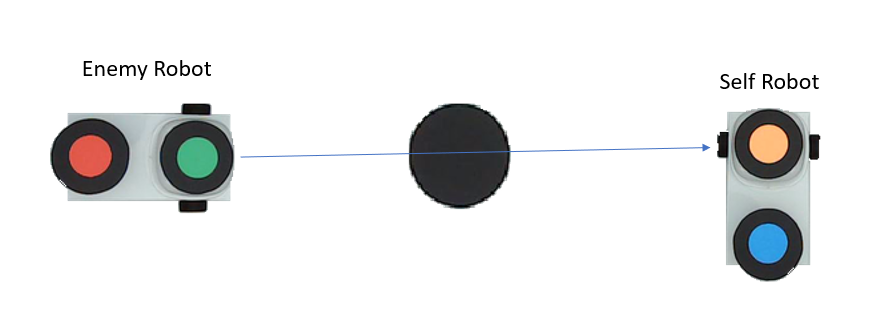
\includegraphics[width=1\textwidth]{images/hiding_strategy.png}
    \caption[hiding strategy]{an example of positions that satisfies the hiding strategy.}\label{hiding_strategy}
\end{figure}

\section{Attacking}
Since there is only one chance to fire the laser, it should fire until there is no obstacle between two robots. In order to do so, attacking robot should chase another robot. 

Method 1:
Move the robot to the position of another robot as soon as possible.

Method 2:
Searching the nearest point that is at the straight line with another robot without an obstacle as shown in figure \ref{attacking_method2}:

\begin{figure}[thb]
    \centering
    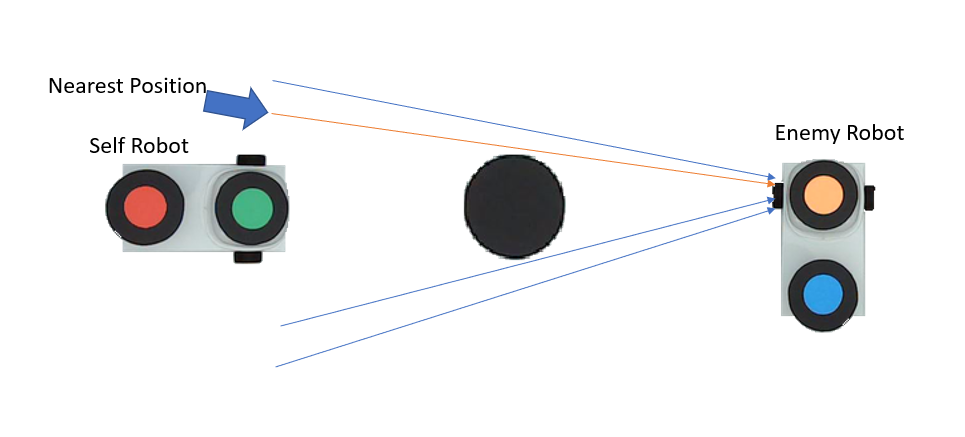
\includegraphics[width=1\textwidth]{images/attacking_method2.png}
    \caption[attacking method]{an example of positions that satisfies the attacking strategy.}\label{attacking_method2}
\end{figure}
